
%%%%%%%%%%%%%%%%%%%%%%% file typeinst.tex %%%%%%%%%%%%%%%%%%%%%%%%%
%
% This is the LaTeX source for the instructions to authors using
% the LaTeX document class 'llncs.cls' for contributions to
% the Lecture Notes in Computer Sciences series.
% http://www.springer.com/lncs       Springer Heidelberg 2006/05/04
%
% It may be used as a template for your own input - copy it
% to a new file with a new name and use it as the basis
% for your article.
%
% NB: the document class 'llncs' has its own and detailed documentation, see
% ftp://ftp.springer.de/data/pubftp/pub/tex/latex/llncs/latex2e/llncsdoc.pdf
%
%%%%%%%%%%%%%%%%%%%%%%%%%%%%%%%%%%%%%%%%%%%%%%%%%%%%%%%%%%%%%%%%%%%


\documentclass[runningheads,a4paper]{llncs}

\usepackage{amssymb}
\setcounter{tocdepth}{3}
\usepackage{graphicx}

\usepackage{url}
\urldef{\mailsa}\path|{timothy.dykes, mel.krokos}@port.ac.uk|    
\newcommand{\keywords}[1]{\par\addvspace\baselineskip
\noindent\keywordname\enspace\ignorespaces#1}


\begin{document}

\mainmatter  % start of an individual contribution

% first the title is needed
\title{Big Data Visualization on the Xeon Phi}

% a short form should be given in case it is too long for the running head
%\titlerunning{Lecture Notes in Computer Science: Authors' Instructions}

% the name(s) of the author(s) follow(s) next
%
% NB: Chinese authors should write their first names(s) in front of
% their surnames. This ensures that the names appear correctly in
% the running heads and the author index.
%
\author{Timothy Dykes\inst{1}
\and Claudio Gheller\inst{2}
\and Marzia Rivi\inst{3}
\and Mel Krokos\inst{1}
}
%
%\authorrunning{Lecture Notes in Computer Science: Authors' Instructions}
% (feature abused for this document to repeat the title also on left hand pages)

% the affiliations are given next; don't give your e-mail address
% unless you accept that it will be published
\institute{   
   University of Portsmouth,
   Portsmouth, U.K.\\
\mailsa\\
\and
  CSCS-ETHZ,
  Lugano, Switzerland\\
  \email{cgheller@cscs.ch}
\and
   University of Oxford,
   Oxford, U.K.\\
   \email{rivi@physics.ox.ac.uk}\\
%\mailsb\\
%\mailsc\\
%\url{http://www.springer.com/lncs}}
}
%
% NB: a more complex sample for affiliations and the mapping to the
% corresponding authors can be found in the file "llncs.dem"
% (search for the string "\mainmatter" where a contribution starts).
% "llncs.dem" accompanies the document class "llncs.cls".
%

%\toctitle{Lecture Notes in Computer Science}
%\tocauthor{Authors' Instructions}
\maketitle


\begin{abstract}
\emph{With the increasing size and complexity of data produced by large scale astrophysical simulations, 
it is important to be able to exploit all available hardware in High performance Computing environments 
for increased throughput and efficiency. We focus on the modification and optimisation of Splotch, a 
scalable data visualization algorithm, to utilise the Xeon Phi, Intel's co-processor based upon the new 
Many Integrated Core architecture. We discuss steps taken to offload data to the co-processor and 
algorithmic modifications to aid faster processing on the many-core architecture and make use of the 
uniquely wide vector capabilities of the device, with accompanying performance results.}

\keywords Big Data, Visualization, Xeon Phi, High Performance Computing, Astrophysics
\end{abstract}


\section{Introduction}
\label{sect:introduction}

Nowadays dealing with big data effectively is a mandatory activity for a rapidly increasing number of scientific communities,
e.g. in environmental, life and health sciences, and in particular in astrophysics. Some of the largest cosmological N-body
simulations can describe the evolution of our universe up to present times by following the behaviour of gravitating matter
represented by hundreds of billions of particles. Performing such simulations often produces time snapshots in the order of tens
of terabytes. This situation can only be exacerbated as supercomputing advances are opening possibilities for simulations
producing snapshots of sizes in the order of petabytes, or even exabytes towards the exascale era.

Large size is not the only challenge posed, it is also essential to effectively extract information from the typically complex datasets. 
Algorithms for data mining and analysis are often highly computationally demanding.
%and in practice unusable on big datasets
%due to time constraints and power limitations. 
Exploration and discovery through visualization can then be an outstanding aid,
e.g. by providing scientists with prompt and intuitive insights enabling them to identify relevant characteristics and thus
define regions of interest within which to apply further time-consuming methods. Additionally, they can be a very effective
way in discovering and understanding correlations, associations and data patterns, or in identifying unexpected behaviours or
even errors. However, visualization algorithms typically require High Performance Computing (HPC) resources to overcome issues
related to rendering large and complex datasets in acceptable timeframes.

Splotch\cite{splotch} is an algorithm for visualizing big particle-based datasets, providing high quality imagery while exploiting
a broad variety of HPC systems such as multi-core processors, multi-node supercomputing systems \cite{splotchmulti}, and
also GPUs \cite{splotchgpu}. The ability to exploit all devices that may be available within a modern HPC system is of paramount
importance towards achieving optimal overall performances. This paper reports on recent developments enabling Splotch to
exploit the capability of the Intel PHI \cite{xeonphi} accelerator, taking advantage of the Many Integrated Core (MIC)
architecture \cite{mic}, which is envisaged to provide, on suitable classes of algorithms, outstanding performance with power
consumption being comparable to standard CPUs. We describe our MIC implementation (Sect. \ref{sect:micsplotch}) focusing on
optimisation issues related to memory usage and data transfers and vectorisation. We then discuss the performance details
(Sect. \ref{sect:results}) of our implementation using a benchmark dataset produced by a Gadget \cite{gadget} N-Body simulation. 
Finally we summarise our experiences and present pointers to future developments.

\section{Background}
\label{sect:background}

\subsection{The Splotch Code}
\label{sect:splotchcode}

Splotch \cite{splotch} is implemented in pure C++ (i.e. no dependencies upon external libraries) and includes several readers 
supporting a number of popular formats for astrophysics. Datasets are converted into the Splotch internal format as they are 
loaded from files. This is followed by preprocessing and rasterisation, and finally rendering. 
Preprocessing can perform ranging, normalization, 
and apply logarithms to particle attributes if necessary. Particles are then roto-translated with reference to supplied 
camera and look-at positions and assigned RGB color values appropriately using externally supplied color maps. For rendering 
pixels, rays are cast along lines of sight, and contributions of all encountered particles are accumulated. The contribution 
of particles is determined by solving the radiative transfer equation \cite{splotchgpu}.

\subsection{Overview of the MIC}
\label{sect:micoverview}

The idea behind MIC is obtaining a massive level of parallelism for increasing throughput performance in power restricted cluster 
environments. To this end Intel's flagship MIC product, the Xeon Phi, contains roughly 60 cores on a single chip, dependent on the 
model. The Xeon Phi acts as a coprocessor for a standard Intel Xeon processor. Programs can be executed natively by logging into 
the device itself, which hosts a Linux micro-OS, or by using the device through one or more MPI processes amongst further processes 
running on the Xeon host. Alternatively users can offload data and portions of code to the coprocessor via a series of pragma 
based extensions available in C++ or FORTRAN.
For a detailed technical description the processor's architecture, the reader is referred to the
Xeon Phi whitepaper \cite{xeonphi}. Here, we give a short overview of its main features.

Each core has access to a 512 KB private fully coherent L2 cache and memory controllers
and the PCIe client logic can access up to 8 GB of GDDR5 memory. A bi-directional ring interconnect
brings these components together. The cores are in-order and up to 4 hardware threads are supported to mitigate
the latencies inherent with in-order execution. The Vector Processor Unit (hereafter VPU) is worth mentioning due to
the utilisation of an innovative 512 bit wide SIMD capability, allowing 16 single precision (SP) or 8 double precision
(DP) floating point operations per cycle. Finally support for fused-multiply-add operations increases this to 32 SP or 16 DP
floating point operations.

\section{Splotch on the MIC}
\label{sect:micsplotch}


\subsection{Implementation}
\label{sect:micimplementation}


The Splotch algorithm can be broken down into a series of distinct phases illustrated by the execution model shown in fig. \ref{fig:exmodel}.
While the executable runs on the Xeon host, data and processing is offloaded to the device via Intel offload clauses.
A double buffered scheme has been implemented using the ability to asynchronously transfer data via a series of signal 
and wait clauses provided by the Intel extensions. This allows to minimise overhead due to transferring data to the device 
for processing, and to facilitate the visualization of datasets potentially much larger than the memory capacity available.

\begin{figure}
\centering
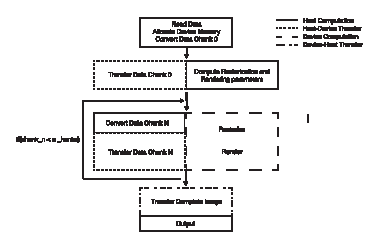
\includegraphics[height=7.0cm]{ExecutionModel}
\caption{Model illustrating execution flow of the new implementation.}
\label{fig:exmodel}
\end{figure}

For rasterization, a highly parallel 3D transform and colorize is performed on a per-particle
basis. Transform parameters are precomputed, as they are identical for each particle, and computation is distributed amongst
threads via an OpenMP parallel for loop. Further tuning enabled this loop to be auto-vectorized by the Intel compiler providing a 
performance boost for this section.

The rendering phase begins with splitting the number of available OpenMP threads into groups, the number of which is dependant on 
a runtime parameter, allocating a buffer per group for the resulting image. The dataset is evenly distributed amongst the 
groups, each rendering to the assigned buffers which are finally accumulated serially. 

Each group image is split into a two dimensional grid of tiles which are distributed amongst threads to avoid race 
conditions where multiple threads attempt to draw to a single pixel simultaneously. For each tile a list is generated 
containing the indices of all particles affecting that tile.

Each thread processes a set number of tiles, rendering the list of particles for each tile. 
In this way pixels are not shared between threads and concurrent accesses are avoided. Finally when all 
chunks of data have been processed and accumulated, the resultant device image is copied back to the host for output. 

\subsection{Optimisation}
\label{sect:micoptimisation}

\subsubsection{Memory Usage and Data Transfer}
\label{sect:memusage}

Cost of dynamic memory allocation on the Phi is relatively high \cite{mem_alloc}, so in order to minimise unnecessary allocations 
buffers are created at the beginning of the program cycle and reused throughout. Use of the MIC\_USE\_2MB\_BUFFERS 
environment variable forces buffers over a particular size to be allocated with 2MB pages rather than the default 4KB, 
which improves data allocation and transfer rates and can benefit performance by potentially reducing page 
faults and TLB (translation look-aside buffer) misses \cite{env_var_buf}. We have performed tests using offload clauses for compiler 
managed memory allocation on the device. To our experience a single process offloading to the device, and reserving large buffers, can
potentially allocate memory roughly 2-2.5x faster having set this environment variable to 64K. The inability to asynchronously 
allocate offload memory means that overheads incurred allocating these buffers cannot be mitigated by overlapping allocation with host activity.

Additionally, overheads in dynamic allocation and data transfer incur a penalty when running a single host process 
offloading to the device. In order to minimise these penalties, we make use of the MPI implementation of Splotch. 
Multiple MPI processes on the host are each allocated a subset of the device threads to exploit. In this way, the device is 
subdivided amongst the host MPI processes allowing for memory and data transfer to occur in parallel providing a noticeable 
performance increase, further details of which are given in sect. \ref{sect:results}.

\subsubsection{Vectorization}
\label{sect:vectorization}

The large 512 bit width SIMD capability of the MIC architecture is exploited through vectorization carried out both 
automatically by the compiler, and manually using Intel Initial Many-Core Instructions (IMCI) \cite{imci}. Firstly the 
particle data structure used in Splotch, a 36 byte structure consisting of 9 fields, was re-examined and converted from an 
array of structures (AoS) to a structure of arrays (SoA). This aids the compiler in automatic vectorization, 
amongst other changes such as ensuring the correct data alignment and modifying loops to be more easily vectorized. 
Such optimisations are described in Intel's Vectorization guide \cite{vectorguide} which, while providing examples for SSE, is also 
applicable to IMCI. Reformatting the data storage method led to a 10\% performance increase in the rasterization phase, 
while the rendering phase was essentially unaffected, leading to a 3\% performance increase of the overall computation. 
The efficacy of this modification may vary, as the rasterization phase affects all particles in the dataset whereas the rendering phase 
affects only those particles viewable within the scene. Hence, if less particles are viewable in the scene the rasterization 
phase will take up a larger portion of the overall time and the performance increase will be more noticeable.

As the rendering phase of the algorithm is complex, and thus unsuitable for automatic vectorization, this is manually 
optimised through use of the Intel intrinsics, which map directly to IMCIs. Drawing consists of additively 
combining a pixel's current RGB values with the contribution from the current particle, which is calculated by 
multiplying the particle color by a scalar contribution value. In order to expedite this process, up to five single 
precision particle RGB values (totalling 480 bits) and five scalar contribution values are packed into two respective 
512 bit vector containers. A third container contains 5 affected pixels, which are written simultaneously using a 
fused multiply-add vector intrinsic, masked in order not to affect the final unused float value in the 16-float 
capable containers.

\subsubsection{Tuning}
\label{sect:tuning}

For relatively datasets where processing time is low, initialisation of the device and OpenMP threads can cause a noticeable overhead. 
The impact of this can be minimised by placing an empty offload clause with empty OpenMP parallel section near to the beginning of 
the program, in order to overlap this overhead while other host activity is occurring, in this case while reading from file. 
Alternatively the environment variable OFFLOAD\_INIT can be set to on\_start to pre-initialise all available MIC devices before the 
program begins execution. 

Various parameters of the algorithm can be tuned to find best performance. Render parameters such as the number of 
thread groups and tile size are set to optimal defaults for the test hardware based on results of scripted tests iterating 
through sets of incremental potential values. These can be modified via a parameter file passed in at runtime for differing 
hardware.

\section{Results}
\label{sect:results}

Performance analysis consisted of running a variety of tests on the “Dommic” facility of the Swiss National Supercomputing Centre, 
Lugano. In this system, each node is based upon a dual socket eight-core Intel Xeon 2670 processor architecture running at 2.6 GHz 
with 32 GB of main system memory. Two Xeon Phi 5110 MIC coprocessors are available per node. 

Tests are carried out using an N-Body simulation performed using Gadget, consisting of roughly 21 million 
particles;  ~10 million dark matter particles, ~10 million baryonic matter particles and ~1 million star particles. 
A 100 frame animation orbiting the dataset is used to measure per-frame timings to produce an image of 800\textsuperscript{2} pixels. 
For performance comparisons, both the host and device code use a tile size parameter of 100 pixels.

In the tests measuring the device performance, we run 8 MPI processes on the host all offloading to the same device, 
as discussed in sect. \ref{sect:memusage} and set thread groups of 15 threads each, which turned out to be the optimal distribution 
for the test system. We use four OpenMP threads per available core to match the four available hardware threads, equating to roughly 240 threads.
OpenMP threads on the host are mapped to one per core.

\begin{figure}
\centering
\begin{minipage}[t]{.45\textwidth}
  \centering
  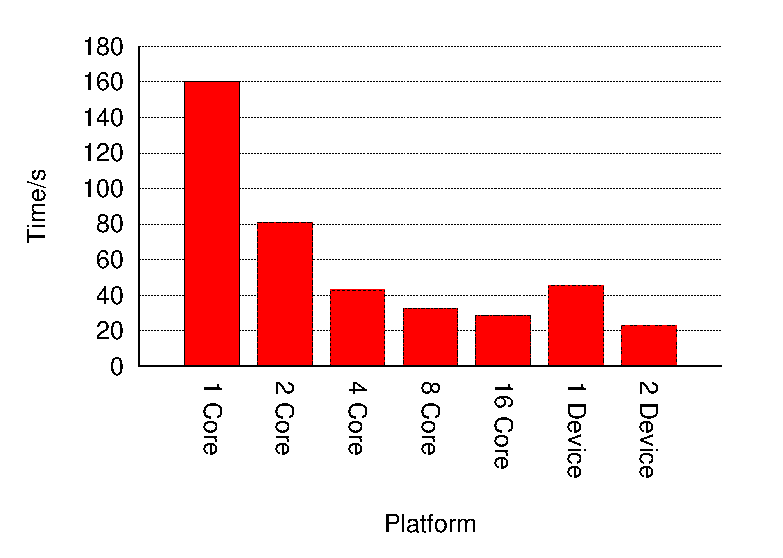
\includegraphics[height=4.0cm]{TotalTime}
\end{minipage}
\begin{minipage}[t]{.45\textwidth}
  \centering
  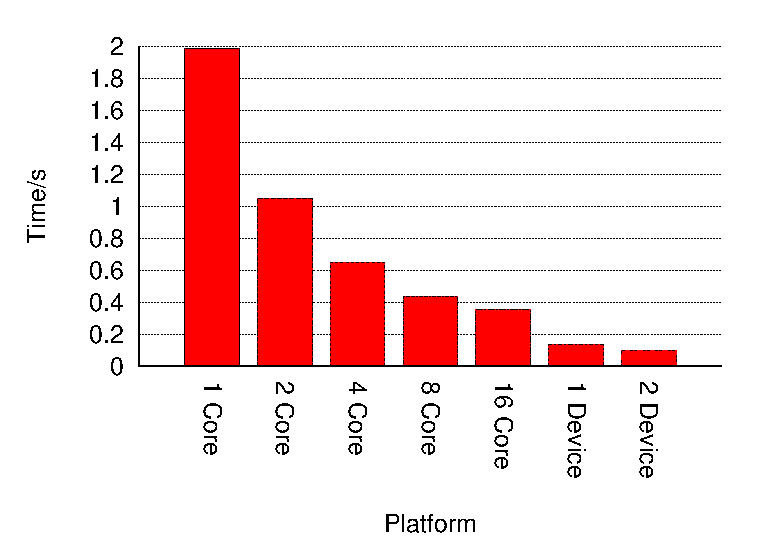
\includegraphics[height=4.0cm]{Rotocol}
\end{minipage}
\caption{\emph{Left:} Per-Frame time for all phases: host OpenMP 1-16 cores vs single and dual Xeon Phi devices.
\emph{Right:} Per-Frame time for rasterization: host OpenMP 1-16 cores vs single and dual Xeon Phi devices.}
\label{fig:timings}
\end{figure}

Fig. \ref{fig:timings} (\emph{left}), describing per frame processing times of the OpenMP host implementation vs dual and single devices, 
shows that use of a single device provides comparable results to 4 cores on the host, while two devices outperform 16 cores by 20\%, due to the 
non-linear scaling of the OpenMP implementation. The additional use of a second device provides a 2x performance improvement for the 
MIC algorithm. Fig. \ref{fig:timings} (\emph{right}) shows the strongest area of improvement, the rasterization phase, with a single 
device outperforming 16 cores roughly 2.5x, with roughly 3x improvement provided by using dual devices. 

Fig. \ref{fig:mpitimes} shows comparison of per-frame processing times using varying numbers of MPI processes on the host, offloading to 
both single and dual devices, against the OpenMP and the MPI implementations of Splotch. Subdividing the available device threads 
amongst host MPI processes allows to transfer data and allocate memory in parallel while also more effectively spreading the 
workload across the device to ensure all threads are working equally. These tests show best performance with 8 and 16 MPI 
processes per device, possibly correspondent to the dual socket 8 core host CPU. It is interesting to note the current offloading model 
with a single device is comparable to 4 cores of the MPI host model, which scales linearly, with two devices comparable to 8 cores, leading 
in the direction of a linear scaling with number of devices.

These results suggest that an optimal usage of the Xeon PHI architecture 
consists of processing the data concurrently by both the multiple host cores, coordinated through the MPI
implementation, and by the device.
Data to be processed by the MIC can be offloaded asynchronously by the various host's cores.
While data from one core is copied to the device, the same core can continue its 
data rendering. At the same time, the MIC can process data already available, previously sent by other cores.

\begin{figure}
\centering
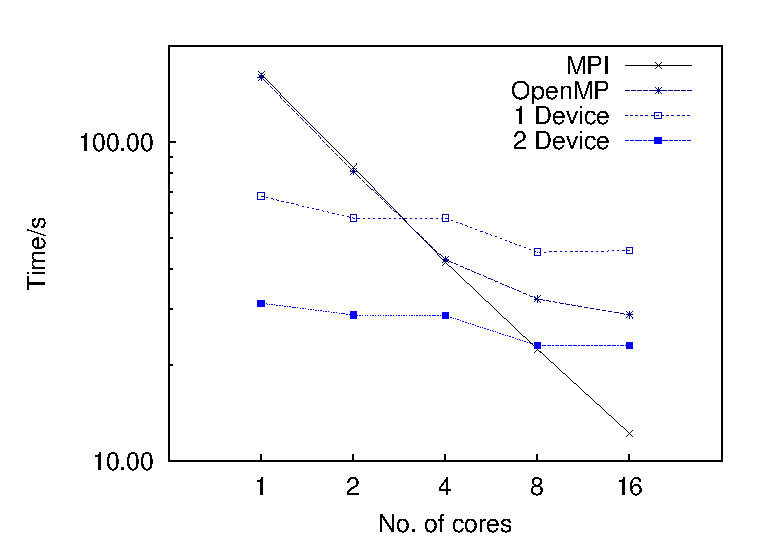
\includegraphics[height=6.0cm]{mpi_omp_mic}
\caption{Per-Frame processing time comparing MPI, OpenMP and MPI offloading to single and dual Xeon Phi devices}
\label{fig:mpitimes}
\end{figure}



\section{Conclusions and Future Work}
\label{sect:conclusions}

The results gathered so far that in some areas of code the MIC architecture excels well beyond the host, 
although in others a fair amount of modification is necessary to gain acceptable performance levels. The use of MPI on the host
provides a considerable performance increase especially for data heavy codes, however launching many MPI processes requires a lengthy 
execution script.

The high performance of the MPI host code indicates implementing an approach running MPI processes on both the host and device 
in order to fully exploit all available processing power may yield a higher overall performance, further work is planned to investigate this.
In addition, work is planned to enable the code to run on multiple host nodes utilising all available devices, with further optimisation and 
testing to be done in order to optimise the double buffered data transfer and processing approach to effectively visualize much larger 
datasets. The ability to use multiple devices across multiple nodes will allow further testing of the scalability of the approach. 
Features provided in the new OpenMP 4.0 specification such as the \textit{teams} construct will enable a OpenMP based approach to 
thread grouping as opposed to the manual method implemented here, if these constructs become supported by the Intel compiler in the future. 

Intel released details of their second generation Xeon Phi product, codenamed “Knights Landing”,  at the International Supercomputing 
Conference 2013 \cite{knightlanding}. One important factor to note is the potential to use this as a standalone CPU rather than a co-processor. 
This is worthy of further investigation as it invites the dismissal of complex and time consuming data transferral methods between 
a host and coprocessor, while retaining the ability to run directly on the host rather than copying executables to an external device.
%  One of the benefits of an offloading model is that work particularly suited to a highly 
% parallelised processing model can be offloaded while unsuitable work can be handled by the more powerful Xeon host 
% cores, disposal of the host would remove this advantage and beg the question of how to handle work that may be 
% inherently unsuitable for a many-core architecture.
 

% \subsubsection{Acknowledgments.}

% Acknowledge people and things here

%The following section shows a sample reference list with entries for
%journal articles \cite{jour}, an LNCS chapter \cite{lncschap}, a book
%\cite{book}, proceedings without editors \cite{proceeding1} and
%\cite{proceeding2}, as well as a URL \cite{url}.
%Please note that proceedings published in LNCS are not cited with their
%full titles, but with their acronyms!

\begin{thebibliography}{4}

\bibitem{splotch}
Dolag, K., Reinecke, M., Gheller, C., Imboden, S.: Splotch: Visualizing Cosmological Simulations. New Journal of Physics, 10(12)  id. 125006 (2008)

\bibitem{splotchmulti} 
Jin, Z., Krokos, M., Rivi, M., Gheller, C., Dolag, K., Reinecke, M.: High-Performance Astrophysical Visualization using Splotch. 
  Procedia Computer Science, 1(1) 1775--1784 (2010)

\bibitem{splotchgpu}
Rivi, M., Gheller, C., Dykes, T., Krokos, M., Dolag, K.:  GPU Accelerated
  Particle Visualisation with Splotch. To appear in Astronomy and Computing (2014)
  
\bibitem{xeonphi} 
Chrysos, G.: Knights Corner, Intel’s first Many Integrated Core (MIC) Architecture Product. 
  Presentation, Hot Chips (2012) 

\bibitem{mic} 
Intel Many Integrated Core Architecture, 
  \url{http://www.intel.com/content/www/us/en/architecture-and-technology/many-integrated-core/intel-many-integrated-core-architecture.html}

\bibitem{mem_alloc} Effective Use of the Intel Compiler's Offload Features.
  Available at \url{http://software.intel.com/en-us/articles/effective-use-of-the-intel-compilers-offload-features}

\bibitem{env_var_buf} 
Intel Corporation: How to Use Huge Pages to Improve Application Performance on Intel Xeon Phi Coprocessor.
  Available at \url{http://software.intel.com/sites/default/files/Large_pages_mic_0.pdf} (2012)

\bibitem{imci} 
Intel Xeon Phi Coprocessor Instruction Set Architecture Reference Manual.
  Available at \url{http://download-software.intel.com/sites/default/files/forum/278102/327364001en.pdf} (2012)

\bibitem{vectorguide} 
A Guide to Vectorization with Intel C++ Compilers.
  Available at \url{http://download-software.intel.com/sites/default/files/8c/a9/CompilerAutovectorizationGuide.pdf} (2012)


\bibitem{gadget} 
The Gadget Code, \url{http://www.mpa-garching.mpg.de/gadget/}

\bibitem{knightlanding} 
Hazra, R.: Driving Industrial Innovation On the Path to Exascale: From Vision to Reality. 
  Presentation, International Supercomputing Conference (2013)


% \bibitem{jour} Smith, T.F., Waterman, M.S.: Identification of Common Molecular
% Subsequences. J. Mol. Biol. 147, 195--197 (1981)

% \bibitem{lncschap} May, P., Ehrlich, H.C., Steinke, T.: ZIB Structure Prediction Pipeline:
% Composing a Complex Biological Workflow through Web Services. In: Nagel,
% W.E., Walter, W.V., Lehner, W. (eds.) Euro-Par 2006. LNCS, vol. 4128,
% pp. 1148--1158. Springer, Heidelberg (2006)

% \bibitem{book} Foster, I., Kesselman, C.: The Grid: Blueprint for a New Computing
% Infrastructure. Morgan Kaufmann, San Francisco (1999)

% \bibitem{proceeding1} Czajkowski, K., Fitzgerald, S., Foster, I., Kesselman, C.: Grid
% Information Services for Distributed Resource Sharing. In: 10th IEEE
% International Symposium on High Performance Distributed Computing, pp.
% 181--184. IEEE Press, New York (2001)

% \bibitem{proceeding2} Foster, I., Kesselman, C., Nick, J., Tuecke, S.: The Physiology of the
% Grid: an Open Grid Services Architecture for Distributed Systems
% Integration. Technical report, Global Grid Forum (2002)

% \bibitem{url} National Center for Biotechnology Information, \url{http://www.ncbi.nlm.nih.gov}

\end{thebibliography}

%(REF7: Procedia Computer Science, 1(1) pp.1775-1784, 2010), and GPUs (REF8: Astronomical Society of the Pacific Conference 
%Series, 475 (ADASS XXII) pp.103-106, 2013; REF2: in preparation). 
%


\end{document}
